\section{Comparison}
\label{sec:comparison}

The simulator has been run with $10$ stations.
All stations are in the communication range of each other, arranged on a ring of radius \SI{3}{\meter}, as shown in \cref {fig:topology}.

\begin{figure}[h!]
	\centering
	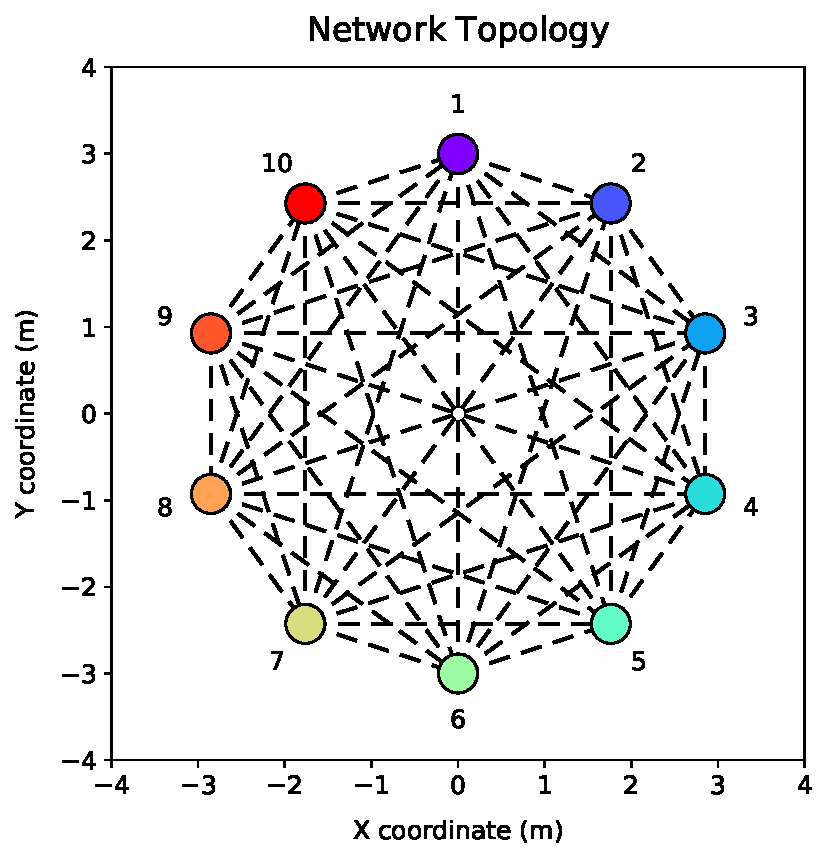
\includegraphics[width=.9\columnwidth]{figures/topology}
	\caption{Network topology used to run the simulations.}
	\label{fig:topology}
\end{figure}

\begin{figure}[t]
	\centering
	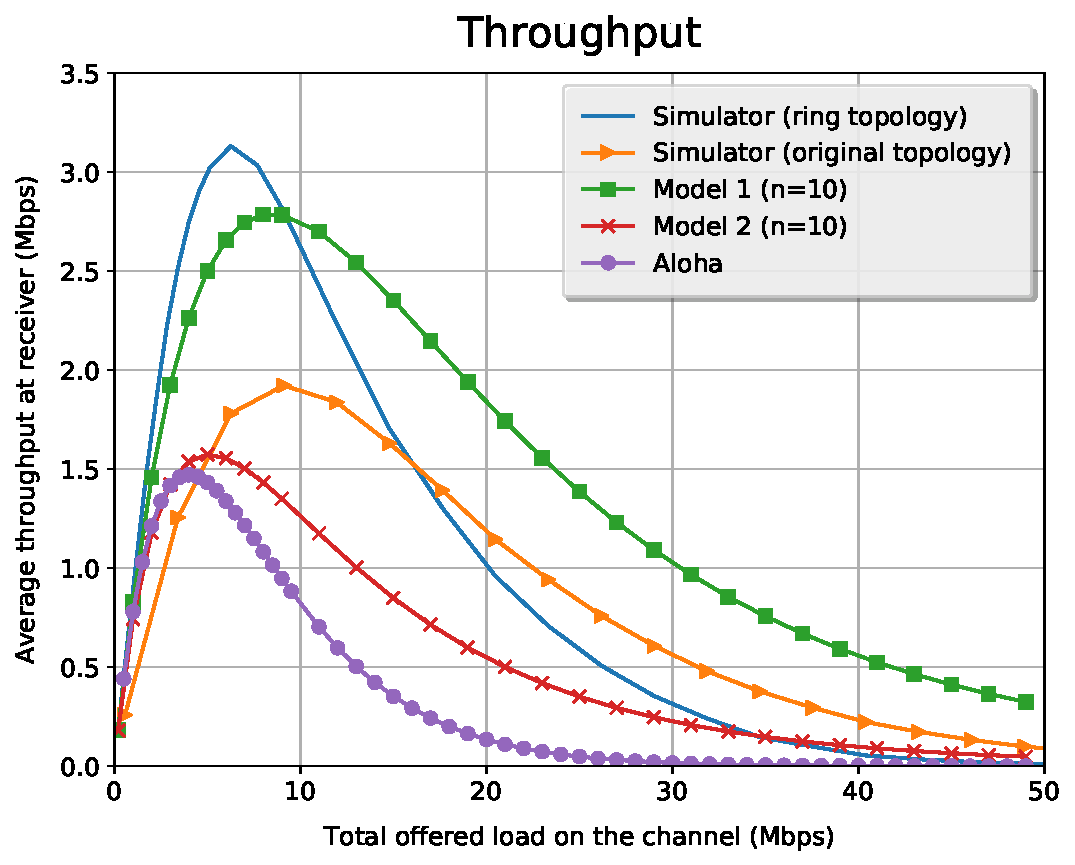
\includegraphics[width=.99\columnwidth]{figures/tr_10}
	\caption{The plot shows the throughput predicted by the different models for a network with 10 stations, compared with the theoretical model for Aloha and the simulator results.}
	\label{fig:tr_10}
\end{figure}

\cref{fig:tr_10} shows the throughput predicted by the different models.
For very low loads, all models behave like the simulator.
For loads near the channel capacity ($8\, Mbps$), the simulator performs better than all models.
This is probably due to the behaviour of the simulated stations:
while a station is receiving a packet, it can not start to transmit.
This helps to avoid collisions and reach a higher throughput.
Models use means which do not take into account this particular behaviour.

The first model predicts a higher throughput than the second one, since it does not differentiate between the state with only one packet (1G) and the state with one packet that was corrupted by some collision (1B).

\cref{fig:tr_1g1b} compares the throughput predicted by the second model for different numbers of stations.
Regardless the number of stations, the maximum throughput is before $10\,Mbps$, near the channel capacity.
With a small number of stations, the maximum throughput is lower, but the throughput at high loads is slightly higher, due to the lower probability of collision.
With a high number of stations, the behaviour is closer to the theoretical model, but with a slightly higher throughput for all loads.

\begin{figure}[t]
	\centering
	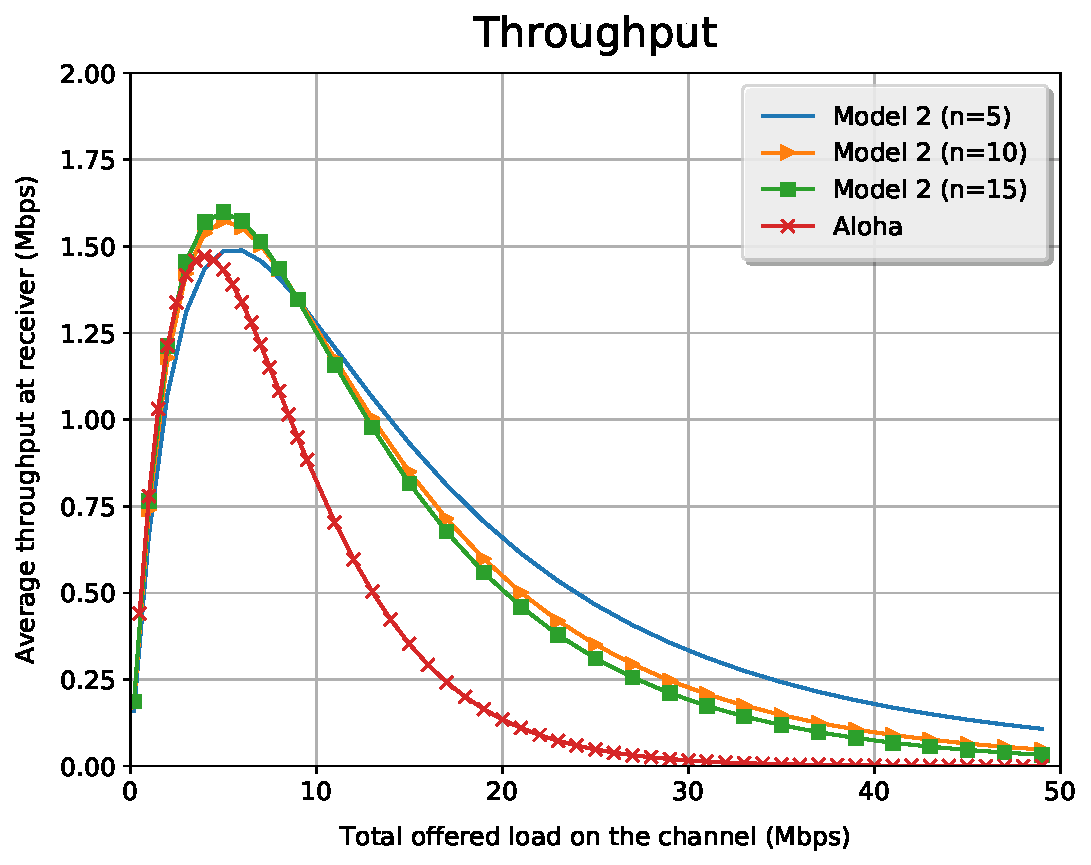
\includegraphics[width=.99\columnwidth]{figures/tr_1g1b}
	\caption{The plot shows the throughput predicted by the second model for different network sized.}
	\label{fig:tr_1g1b}
\end{figure}

\cref{fig:cr_10} shows the collision rate predicted by the different models.
The first model has a lower collision rate than the second one, that also justify the higher throughput.
The collision rate of the simulator at low loads is smaller than the second model, then gets slightly higher for medium and high loads.

\begin{figure}[t]
	\centering
	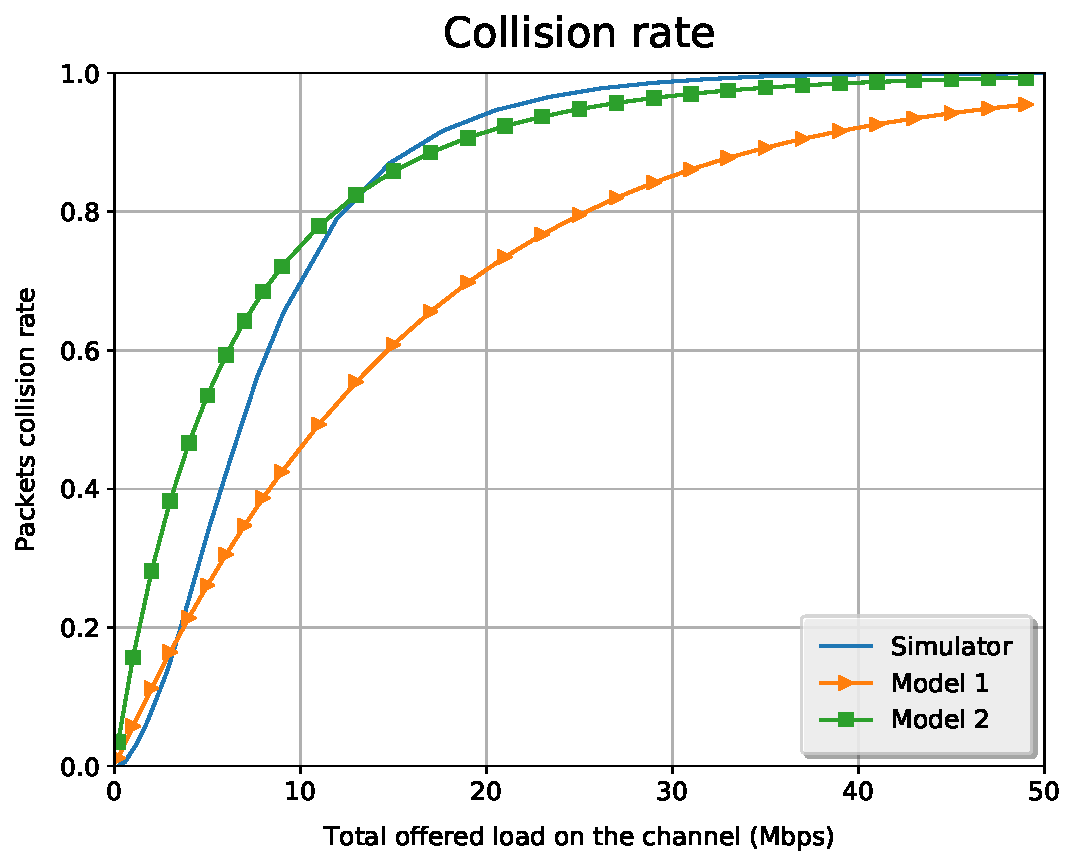
\includegraphics[width=.99\columnwidth]{figures/cr_10}
	\caption{The plot shows the collision rate predicted by the different for a network with 10 stations, compared with the simulator results.}
	\label{fig:cr_10}
\end{figure}

